\chapter{Ek Çözümlü Problemler ve İpuçları}

Önceki bölümlerde kurduğumuz teorik temeller, kurallar ve algoritmalar; sınav soruları karşısında somut birer çözüm aracına dönüştüklerinde anlam kazanır. Bir problemi ilk denemede çözememek bir eksiklik değil, zihnimizde henüz kurulmamış bir bağlantıyı keşfetme fırsatıdır. \textbf{Bu bölümdeki problemler, önceki bölümlerde öğrendiğimiz araçları pekiştirmek için hazırlanmış ek çözümlü sorulardır}; konu başlıklarına göre (sayma, sayılar teorisi ve algoritma) üç kısma ayrılmıştır. Her çözümün sonunda benzer sorularda yol gösterecek ipuçları da veriyoruz.

Çözümlerde yalnızca doğru yanıtı vermekle yetinmeyip bir yarışmacının soruya yaklaşırken yakalaması gereken ipuçlarını, olası tuzakları ve sonuca ulaştıran akıl yürütme adımlarını öne çıkarıyoruz.

\section{Ek Problemler: İleri Sayma ve Kombinatorik}

Sayma problemleri ilk bakışta sade görünse de kısıtlar arttıkça doğrudan listelemek olanaksız hale gelir. Bu kısımda kısıtlı dizilimler (Bölüm 4), içerme-dışarma ilkesi (Bölüm 8), ayraç yöntemi (Bölüm 5) ve güvercin yuvası ilkesi (Bölüm 7) gibi tekniklerin tipik uygulamaları üzerinde duruyoruz.

\subsection{Kısıtlı Sıralama ve Özdeş Nesneler}

\begin{example}
$\{1, 2, 3, 4, 5, 6, 7\}$ kümesinin elemanları kullanılarak yazılabilecek tüm 7 basamaklı, rakamları tekrarsız sayıların kaç tanesinde tek rakamlar kendi aralarında küçükten büyüğe sıralı (soldan sağa $1, 3, 5, 7$ sırasında), fakat çift rakamlar da kendi aralarında büyükten küçüğe sıralı (soldan sağa $6, 4, 2$ sırasında) yer alır?
\end{example}

\begin{proof}[Çözüm]
Soruda 7 farklı basamağın yerleştirilmesi isteniyor. Eğer tek basamaklar ($1, 3, 5, 7$) ve çift basamaklar ($2, 4, 6$) rastgele dağılsaydı $7!$ farklı durum oluşurdu. Ancak iki grup üzerinde de kesin bir sıra şartı vardır. Teklerin kendi aralarındaki $1 < 3 < 5 < 7$ sıralaması tek bir biçimde mümkündür; benzer şekilde çiftlerin $6 > 4 > 2$ sıralaması da tek bir dizilim verir. Dolayısıyla bir grubun yerlerini seçtiğimiz anda o grubun elemanlarının yazılış sırası tamamen belirlenir; geriye kalan yerlere de diğer grubun elemanları zorunlu olarak tek biçimde yerleşir.

Adım adım kuralım:
\begin{enumerate}
    \item Toplam 7 basamak pozisyonumuz var: $\_ \_ \_ \_ \_ \_ \_$.
    \item Bu 7 pozisyondan 4 tanesini tek sayılar için seçelim. Bu seçim kombinasyon ile yapılır:
    \[
    \binom{7}{4} = \frac{7 \times 6 \times 5 \times 4}{4 \times 3 \times 2 \times 1} = 35.
    \]
    \item Seçilen 4 yere tek sayılar $1, 3, 5, 7$ kural gereği yalnızca \textbf{1 farklı şekilde} (küçükten büyüğe) yerleştirilebilir.
    \item Geriye kalan $7 - 4 = 3$ pozisyona çift sayılar yerleşmelidir. Bu 3 pozisyon için çift sayıların sırası da büyükten küçüğe ($6, 4, 2$) olacak şekilde \textbf{1 farklı biçimde} zorunludur.
\end{enumerate}

Çarpma kuralı uyarınca toplam geçerli dizilim sayısı:
\[
\binom{7}{4} \times 1 \times 1 = 35
\]
olarak bulunur.

\textbf{Alternatif Bakış (Tekrarlı Permütasyon Sezgisi):}
Dört tek sayıyı özdeş $T$ simgesiyle, üç çift sayıyı özdeş $C$ simgesiyle temsil edelim. $T, T, T, T, C, C, C$ harflerinin diziliş sayısı $\frac{7!}{4!3!} = 35$'tir. Herhangi bir dizilimde (örneğin $T C T T C C T$) soldan sağa ilk $T$'ye $1$, ikincisine $3$, üçüncüsüne $5$, dördüncüsüne $7$; ilk $C$'ye $6$, ikincisine $4$, üçüncüsüne $2$ yazmak zorundayız. Dolayısıyla özdeş harf dizilimleri ile aranan sayılar arasında birebir eşleme (Bölüm 10) vardır.
\end{proof}

\textbf{En sık yapılan hata:} Çiftlerin ve teklerin sıralamasını da hesaba katıp sonucu yanlışlıkla $\binom{7}{4} \times 4! \times 3! = 7!$ ile karıştırmaktır. Sıralama önceden belirlenmişse o elemanlar arasındaki permütasyon serbestliği $1$'e düşer.

\subsection{İçerme-Dışarma İlkesi ile Kısıtlı Sayma}

\begin{example}
$A = \{1, 2, 3, 4, 5\}$ kümesinden $B = \{1, 2, 3\}$ kümesine tanımlanabilecek örten (surjective) fonksiyonların sayısını bulunuz.
\end{example}

\begin{proof}[Çözüm]
Bir fonksiyonun örten olması, değer kümesindeki her bir elemanın en az bir kez görüntü olarak seçilmesi demektir. Her elemanın seçildiği durumları doğrudan saymak yerine, Bölüm 8'de gördüğümüz içerme-dışarma ilkesinden yararlanarak örten olmayan durumları tüm durumlardan çıkarmak çok daha pratiktir. Değer kümesindeki en az bir eleman boşta kalırsa fonksiyon örten olamaz.

Tüm fonksiyonların evrensel kümesini $U$, $B$ kümesindeki $i$ elemanının görüntü kümesinde yer almadığı fonksiyonlar kümesini $A_i$ ($i \in \{1, 2, 3\}$) ile gösterelim.

\begin{enumerate}
    \item \textbf{Evrensel kümenin boyutu $|U|$:}
    Tanım kümesindeki 5 elemanın her biri için $B$'de 3 seçenek vardır:
    \[
    |U| = 3^5 = 243.
    \]

    \item \textbf{Bir elemanın boşta kaldığı durumlar ($|A_i|$):}
    Belirli bir eleman (örneğin $1$) seçilmezse, tüm elemanlar kalan 2 elemana gitmelidir:
    \[
    |A_i| = 2^5 = 32.
    \]
    $B$'de 3 eleman olduğundan $\binom{3}{1} = 3$ farklı durum vardır:
    \[
    \sum_{i} |A_i| = \binom{3}{1} \times 2^5 = 3 \times 32 = 96.
    \]

    \item \textbf{İki elemanın aynı anda boşta kaldığı durumlar ($|A_i \cap A_j|$):}
    Belirli iki eleman (örneğin $1$ ve $2$) seçilmezse, tüm 5 eleman kalan tek elemana gitmek zorundadır:
    \[
    |A_i \cap A_j| = 1^5 = 1.
    \]
    $\binom{3}{2} = 3$ ikili vardır:
    \[
    \sum_{i < j} |A_i \cap A_j| = \binom{3}{2} \times 1^5 = 3 \times 1 = 3.
    \]

    \item \textbf{Üç elemanın birden boşta kaldığı durumlar ($|A_1 \cap A_2 \cap A_3|$):}
    Fonksiyon tanımı gereği görüntü kümesi boş olamaz; 0 elemana giden fonksiyon sayısı $0^5 = 0$'dır.
\end{enumerate}

İçerme-dışarma ilkesi gereğince, en az bir elemanı dışarıda bırakan fonksiyonların sayısı:
\[
|A_1 \cup A_2 \cup A_3| = \sum |A_i| - \sum |A_i \cap A_j| + |A_1 \cap A_2 \cap A_3| = 96 - 3 + 0 = 93.
\]
Dolayısıyla, örten fonksiyon sayısı:
\[
|U| - |A_1 \cup A_2 \cup A_3| = 243 - 93 = 150
\]
olarak hesaplanır.
\end{proof}

\subsection{Ayraç (Stars and Bars) Yöntemi}

\begin{example}
$x_1 + x_2 + x_3 + x_4 = 18$ denklemini sağlayan ve $x_1 \ge 1$, $x_2 \ge 2$, $x_3 \ge 0$, $x_4 \ge 3$ koşullarına uyan kaç farklı $(x_1, x_2, x_3, x_4)$ tam sayı dörtlüsü vardır?
\end{example}

\begin{proof}[Çözüm]
Bölüm 5'te ele aldığımız ayraç yöntemi, değişkenlerin negatif olmadığı ($y_i \ge 0$) durumlar için geçerlidir. Değişkenlerin alt sınırları birbirinden farklı olduğunda en doğal ilk hamle, değişken değiştirerek her birinin alt sınırını $0$'a çekmektir. Bu işlem, ceplerinde belirli miktarda para bulunması gereken kişilere bu miktarı peşinen dağıtmaya benzer.

Yeni değişkenleri tanımlayalım:
\begin{align*}
y_1 &= x_1 - 1 \ge 0 \implies x_1 = y_1 + 1, \\
y_2 &= x_2 - 2 \ge 0 \implies x_2 = y_2 + 2, \\
y_3 &= x_3 - 0 \ge 0 \implies x_3 = y_3, \\
y_4 &= x_4 - 3 \ge 0 \implies x_4 = y_4 + 3.
\end{align*}

Bu ifadeleri orijinal denklemde yerine yazalım:
\[
(y_1 + 1) + (y_2 + 2) + y_3 + (y_4 + 3) = 18
\]
\[
y_1 + y_2 + y_3 + y_4 + 6 = 18 \implies y_1 + y_2 + y_3 + y_4 = 12.
\]

Şimdi problem, $12$ özdeş nesneyi negatif olmayan 4 değişkene ($y_1, y_2, y_3, y_4 \ge 0$) dağıtma problemine dönüştü. Ayraç teoremine göre, $n$ özdeş nesneyi $k$ farklı kutuya paylaştırmak için $n$ nesne ve $k - 1$ ayraç kullanılır:
\[
\binom{n + k - 1}{k - 1} = \binom{12 + 4 - 1}{4 - 1} = \binom{15}{3}.
\]
Kombinasyonu hesaplayalım:
\[
\binom{15}{3} = \frac{15 \times 14 \times 13}{3 \times 2 \times 1} = 5 \times 7 \times 13 = 455.
\]
Demek ki koşulları sağlayan 455 farklı tam sayı çözümü vardır.
\end{proof}

\textbf{En sık yapılan hata:} Alt sınırları pozitif olan değişkenleri sıfıra çekerken sağ taraftan toplamı çıkarmak yerine toplamak veya sınırları yanlış eksiltmektir (örneğin $x_1 \ge 1$ için $1$ eksiltmek yerine $0$ almak).

\subsection{Güvercin Yuvası İlkesi}

\begin{example}
Kenar uzunluğu $1$ birim olan bir eşkenar üçgenin içerisine rastgele 5 nokta yerleştiriliyor. Bu noktalardan en az ikisi arasındaki mesafenin $\le \frac{1}{2}$ birim olduğunu kanıtlayınız.
\end{example}

\begin{proof}[Çözüm]
Soruda verilen 5 nokta ve aranan $\le \frac{1}{2}$ mesafesi, Bölüm 7'de incelediğimiz Güvercin Yuvası İlkesi'ni akla getirir. İlkeyi uygulayabilmek için üçgeni öyle bölgelere ayırmalıyız ki bölge sayısı nokta sayısından az (yani en fazla 4) olsun ve her bir bölgedeki herhangi iki nokta arasındaki mesafe en fazla $\frac{1}{2}$ birim kalabilsin.

\begin{figure}[htbp]
\centering
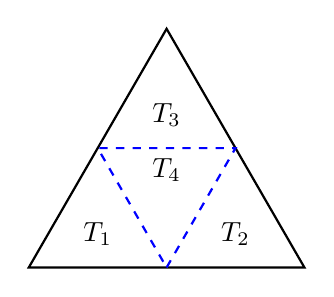
\begin{tikzpicture}[scale=3.5]
  % Büyük üçgen
  \coordinate (A) at (0,0);
  \coordinate (B) at (1,0);
  \coordinate (C) at (0.5,{sqrt(3)/2});
  
  \draw[thick] (A) -- (B) -- (C) -- cycle;
  
  % Kenar orta noktaları
  \coordinate (M_AB) at (0.5,0);
  \coordinate (M_BC) at (0.75,{sqrt(3)/4});
  \coordinate (M_CA) at (0.25,{sqrt(3)/4});
  
  % İç üçgen çizgileri
  \draw[dashed, thick, blue] (M_AB) -- (M_BC) -- (M_CA) -- cycle;
  
  % Bölge etiketleri
  \node at (0.25, 0.12) {$T_1$};
  \node at (0.75, 0.12) {$T_2$};
  \node at (0.5, {sqrt(3)/4 + 0.12}) {$T_3$};
  \node at (0.5, {sqrt(3)/4 - 0.08}) {$T_4$};
\end{tikzpicture}
\caption{Eşkenar üçgenin 4 eş parçaya bölünmesi}
\end{figure}

Kenar uzunluğu $1$ birim olan eşkenar üçgenin her kenarının orta noktasını birleştirelim. Bu işlem büyük üçgeni, kenar uzunluğu $\frac{1}{2}$ birim olan 4 adet eşkenar üçgene ($T_1, T_2, T_3, T_4$) böler.

\begin{enumerate}
    \item \textbf{Yuvalar:} 4 küçük eşkenar üçgen.
    \item \textbf{Güvercinler:} Üçgen içine yerleştirilen 5 nokta.
\end{enumerate}

Güvercin yuvası ilkesi uyarınca, 5 nokta 4 yuvaya dağıtıldığında en az bir küçük üçgenin içine en az $\lceil 5/4 \rceil = 2$ nokta düşmek zorundadır.

Kenar uzunluğu $\frac{1}{2}$ olan kapalı bir eşkenar üçgenin içindeki veya sınırındaki herhangi iki nokta arasındaki maksimum uzaklık (üçgenin çapı), iki köşe arasındaki uzaklıktır; o da tam olarak $\frac{1}{2}$ birimdir.

Dolayısıyla aynı küçük üçgene düşen bu iki nokta arasındaki mesafe en fazla $\frac{1}{2}$ birim olabilir. İspat tamamlanır.
\end{proof}

\section{Ek Problemler: Sayılar Teorisi ve Problem Çözme Teknikleri}

Sayılar teorisinde saf aritmetik manipülasyonlar tek başına yeterli olmaz; parite (Bölüm 17), invaryantlar (Bölüm 18), modüler kongrüanslar (Bölüm 14) ve uç değer ilkesi (Bölüm 19) gibi yöntemler birlikte kullanılır.

\subsection{Modüler Aritmetik ve Bölünebilme}

\begin{example}
$2^{2026} + 3^{2026}$ sayısının 7 ile bölümünden kalan kaçtır?
\end{example}

\begin{proof}[Çözüm]
Büyük üslerle karşılaştığımızda iki temel yol öne çıkar: Bölüm 14'te gördüğümüz üzere tabanın kuvvetlerinin mod $m$'deki periyodunu belirlemek ya da aynı bölümde ispatladığımız Fermat'nın Küçük Teoremi'nden yararlanmak. 7 asal sayı olduğundan, $\gcd(a, 7) = 1$ koşulunu sağlayan her $a$ için Fermat Teoremi $a^{7-1} = a^6 \equiv 1 \pmod 7$ denkliğini verir.

Üs olan $2026$'yı mod $6$'da inceleyelim:
\[
2026 = 6 \times 337 + 4 \implies 2026 \equiv 4 \pmod 6.
\]

Fermat'nın Küçük Teoremi uyarınca:
\[
2^6 \equiv 1 \pmod 7 \quad \text{ve} \quad 3^6 \equiv 1 \pmod 7.
\]

O halde:
\[
2^{2026} = (2^6)^{337} \times 2^4 \equiv 1^{337} \times 2^4 \equiv 16 \pmod 7.
\]
$16 = 2 \times 7 + 2 \implies 16 \equiv 2 \pmod 7$. Demek ki $2^{2026} \equiv 2 \pmod 7$.

Şimdi $3^{2026}$ terimini hesaplayalım:
\[
3^{2026} = (3^6)^{337} \times 3^4 \equiv 1^{337} \times 3^4 \equiv 81 \pmod 7.
\]
$81 = 11 \times 7 + 4 \implies 81 \equiv 4 \pmod 7$. Demek ki $3^{2026} \equiv 4 \pmod 7$.

Toplarsak:
\[
2^{2026} + 3^{2026} \equiv 2 + 4 \equiv 6 \pmod 7.
\]
Sonuç olarak, verilen sayının 7 ile bölümünden kalan 6'dır.
\end{proof}

\subsection{Değişmezler (Invariants) ve Parite}

\begin{example}
Bir tahtada 1'den 20'ye kadar olan tam sayılar yazılıdır: $1, 2, 3, \dots, 20$. Bir öğrenci her adımda tahtadan rastgele iki $a$ ve $b$ sayısını silip yerlerine $|a - b|$ sayısını yazıyor. Tahtada tek bir sayı kalana kadar bu işleme devam ediliyor. Son kalan sayı $0$ olabilir mi?
\end{example}

\begin{proof}[Çözüm]
İşlem adımları serbesttir; hangi iki sayının silineceği önceden kestirilemez. Bu tür süreç problemlerinde her adımda korunan bir özellik, yani bir invaryant (Bölüm 18) aramak gerekir. Sayıların toplamının tekliğini veya çiftliğini, yani paritesini (Bölüm 17) inceleyelim.

İki sayı $a$ ve $b$ silinip yerine $|a - b|$ yazıldığında, tahtadaki sayıların toplamı nasıl değişir?
Eski toplam $S_{\text{eski}}$ olsun. Yeni toplam:
\[
S_{\text{yeni}} = S_{\text{eski}} - a - b + |a - b|.
\]
Toplamdaki değişim miktarı $\Delta = S_{\text{eski}} - S_{\text{yeni}}$:
\[
\Delta = a + b - |a - b|.
\]
Biliyoruz ki her $a, b \in \mathbb{Z}$ için:
\[
a + b \equiv a - b \equiv |a - b| \pmod 2.
\]
Çünkü iki sayının farkı ile toplamının paritesi aynıdır ($(a+b) - (a-b) = 2b \equiv 0 \pmod 2$).

Dolayısıyla:
\[
\Delta = (a + b) - |a - b| \equiv |a - b| - |a - b| \equiv 0 \pmod 2.
\]
Bu önemli bir tespittir: Her adımda tahtadaki sayıların toplamı çift bir sayı kadar azalır. Yani toplamın mod 2'deki değeri, başka bir deyişle \textbf{paritesi bir invaryanttır}.

Şimdi başlangıçtaki sayıların toplamını hesaplayalım:
\[
S_0 = 1 + 2 + 3 + \dots + 20 = \frac{20 \times 21}{2} = 210.
\]
$210 \equiv 0 \pmod 2$ (başlangıç toplamı çifttir).

Değişmezlik kuralı gereğince tahtada son kalan tek sayı $X$ ise:
\[
X \equiv S_0 \equiv 0 \pmod 2
\]
olmalıdır. $0$ çift bir sayı olduğundan ($0 \equiv 0 \pmod 2$), parite argümanı $0$'ı doğrudan elemez. Ancak soru ``0 olabilir mi?'' diye soruyor. Bir an durup daha derine bakalım:

Başlangıç kümesindeki tek sayıların adedine bakalım:
$\{1, 3, 5, 7, 9,$ $11,$ $13,$ $15,$ $17,$ $19\} \implies 10$ adet tek sayı vardır.
İki sayı seçildiğinde:
\begin{itemize}
    \item İkisi de tek ise: $|T_1 - T_2| = \text{çift}$. Tek sayı adedi 2 azalır.
    \item Biri tek, biri çift ise: $|T - C| = \text{tek}$. Tek sayı adedi değişmez.
    \item İkisi de çift ise: $|C_1 - C_2| = \text{çift}$. Tek sayı adedi değişmez.
\end{itemize}
Görüldüğü üzere tek sayıların sayısı her adımda ya 0 ya da 2 azalır. Başlangıçta 10 adet tek sayı olduğundan, adımların sonucunda tek sayı adedi $10 \to 8 \to \dots \to 0$ olabilir. Dolayısıyla son kalan sayı çift olmalıdır; 0 da çifttir.

Peki gerçekten 0 elde edilebilir mi?
Sayıları ardışık çiftler halinde gruplayalım:
$(1,2), (3,4), (5,6), \dots, (19,20)$.
Her çifte işlem uygularsak $|k - (k+1)| = 1$ elde edilir.
Böylece tahtada 10 tane $1$ kalır: $1, 1, 1, 1, 1, 1, 1, 1, 1, 1$.
Şimdi bu 1'leri ikişer ikişer eşleyip çıkarırsak:
$|1 - 1| = 0$ elde edilir. 5 adet $0$ kalır.
Sıfırların farkı daima $0$'dır: $|0 - 0| = 0$.
Sonuç olarak tek kalan sayı $0$ \textbf{olabilir}.
\end{proof}

\textbf{En sık yapılan hata:} Parite invaryantını bulunca incelemeyi bırakmaktır. Toplamın çift çıkması sonucun kesinlikle 0 olabileceğini tek başına kanıtlamaz; geçerli bir işlem dizisi (yapıcı örnek / kurgu) sunulmalıdır.

\subsection{Uç Değer İlkesi (Extremal Principle)}

\begin{example}
Düzlemde sonlu sayıda nokta bulunmaktadır. Bu noktaların oluşturduğu tüm ikili mesafeler birbirinden farklıdır. Her nokta, kendisine en yakın olan noktaya bir ok çiziyor. Hiçbir noktanın beşten fazla ok alamayacağını kanıtlayınız.
\end{example}

\begin{proof}[Çözüm]
Bölüm 2'deki çelişkiyle ispat ve Bölüm 19'daki uç değer ilkesini birleştirelim. Bir noktanın en az 3 ok aldığını varsayıp bu noktaya gelen okların uçlarındaki noktalar arasındaki açıları ve mesafeleri inceleyelim.

Bir $P$ noktasına $A, B, C$ gibi en az üç farklı noktadan ok gelmiş olsun.
Bu durum, $A$'ya en yakın noktanın $P$, $B$'ye en yakın noktanın $P$, $C$'ye en yakın noktanın $P$ olduğu anlamına gelir:
\[
|AP| < |AB| \quad \text{ve} \quad |AP| < |AC|,
\]
\[
|BP| < |BA| \quad \text{ve} \quad |BP| < |BC|,
\]
\[
|CP| < |CA| \quad \text{ve} \quad |CP| < |CB|.
\]

$P$ noktasının etrafındaki $A, B, C$ noktalarını $P$'ye göre saat yönünde sıralayalım. Bu üç noktadan en az iki komşu olanı arasındaki açıya bakalım. $P$ merkezli açılardan en az biri:
\[
\angle APB + \angle BPC + \angle CPA = 360^\circ
\]
olduğundan, güvercin yuvası mantığıyla (Bölüm 7) bu açılardan en az biri $\le \frac{360^\circ}{3} = 120^\circ$ olmak zorundadır. Ancak daha da dar bir sınır vardır.

$A$ ve $B$ noktalarını ve $PAB$ üçgenini ele alalım:
$A$'nın $P$'ye olan mesafesi $|AP|$, $B$'ye olan mesafesi $|AB|$'den küçüktür ($|AP| < |AB|$).
Aynı şekilde $B$'nin $P$'ye mesafesi $|BP|$, $A$'ya mesafesinden küçüktür ($|BP| < |AB|$).

Dolayısıyla $PAB$ üçgeninde en uzun kenar kesinlikle $AB$ kenarıdır:
\[
|AB| > |AP| \quad \text{ve} \quad |AB| > |BP|.
\]

Bir üçgende en büyük kenarın karşısındaki açı en büyük açıdır. Dolayısıyla:
\[
\angle APB > \angle PAB \quad \text{ve} \quad \angle APB > \angle PBA.
\]
Bir üçgenin iç açıları toplamı $180^\circ$ olduğundan:
\[
\angle APB > 60^\circ
\]
olmak zorundadır! Çünkü eğer $\angle APB \le 60^\circ$ olsaydı, diğer iki açıdan en az biri $\ge 60^\circ \ge \angle APB$ olurdu ki bu da $AB$'nin en büyük kenar olmasıyla çelişirdi.

Demek ki $P$'ye ok gönderen herhangi iki noktanın $P$ merkezinde oluşturduğu açı \textbf{kesinlikle $60^\circ$'den büyük} olmalıdır:
\[
\theta_{i,j} > 60^\circ.
\]

Eğer bir noktaya $k$ tane ok geliyorsa:
\[
360^\circ = \sum_{i=1}^k \theta_i > k \times 60^\circ \implies k < \frac{360^\circ}{60^\circ} = 6.
\]
$P$'ye ok gönderen iki nokta $A, B$ ise $|AB| > \max(|PA|, |PB|)$ olduğundan $AB$ üçgenin en uzun kenarıdır; en uzun kenarın karşısındaki açı en büyük açı olduğundan $\angle APB > 60^\circ$'dir.

Dolayısıyla $P$'ye $k$ ok geliyorsa bu okların $P$ merkezinde oluşturduğu $k$ açının her biri $60^\circ$'den büyüktür ve toplamları $360^\circ$'dir:
\[
k \times 60^\circ < 360^\circ \implies k < 6 \implies k \le 5.
\]

Bu sınır keskindir: $P$'nin çevresine $72^\circ$ arayla yerleştirilen 5 nokta, yarıçapları birbirinden çok az farklı seçildiğinde hem $P$'yi en yakın komşu olarak seçer hem de aralarındaki tüm ikili mesafeler birbirinden farklı kalır; yani 5 ok gerçekten mümkündür.
\end{proof}

\section{Ek Problemler: Algoritmalar ve C Programlama}

Algoritmik sorularda teorik matematiksel analizin yanı sıra bellek modelleri, işaretçi aritmetiği (Bölüm 31), asimptotik karmaşıklık ($O$, Bölüm 21) ve sınır durumların C dilinde doğru kodlanması belirleyicidir.

\subsection{Cevaba İkili Arama (Binary Search on Answer)}

\begin{example}
Elimizde $n$ adet tahta parçası vardır; $i$'inci tahtanın uzunluğu $L[i]$ birimdir. Bu tahtaları keserek eşit uzunlukta en az $k$ adet küçük tahta parçası elde etmek istiyoruz. Elde edilebilecek bir parçanın tam sayı cinsinden \textbf{en büyük} uzunluğunu $O(n \log(\max L))$ zaman karmaşıklığında bulan C fonksiyonunu yazınız.
\end{example}

\begin{proof}[Çözüm]
``En büyük uzunluk nedir?'' sorusunu doğrudan çözmek yerine Bölüm 24'te gördüğümüz gibi bir karar problemine dönüştürelim: ``Her bir parçanın uzunluğu $x$ birim olacak şekilde en az $k$ parça kesilebilir mi?''
Eğer parça boyu $x$ iken $k$ parça kesilebiliyorsa, $x$'ten daha küçük her değer için de bu mümkündür. Eğer $x$ boyunda kesilemiyorsa, $x$'ten büyük hiçbir boyda kesilemez. Bu özellik arama uzayının \textbf{monoton} olduğunu gösterir. Monotonluk sağlandığı için doğrusal arama ($O(\max L)$) yerine ikili arama ($O(\log(\max L))$) uygulayabiliriz.

$x$ uzunluğunda parçalar kesildiğinde $L[i]$ boyundaki tahtadan $\lfloor L[i] / x \rfloor$ parça elde edilir. Toplam parça sayısı:
\[
f(x) = \sum_{i=0}^{n-1} \left\lfloor \frac{L[i]}{x} \right\rfloor.
\]
Karar fonksiyonumuz: $f(x) \ge k$ ise geçerli (true), aksi halde geçersiz (false).

İkili arama aralığımız $[1, \max(L)]$ olacaktır.

Aşağıdaki C kodunda bu mantık eksiksiz şekilde uygulanmıştır:

\begin{lstlisting}[language=CTemel]
#include <stdio.h>

/* Karar fonksiyonu: x uzunlugunda en az k parca cikar mi? */
int kesilebilir_mi(const int L[], int n, int k, int x) {
    if (x <= 0) return 1;
    long long toplam_parca = 0;
    for (int i = 0; i < n; i++) {
        toplam_parca += (L[i] / x);
        if (toplam_parca >= k) {
            return 1; /* Erken sonlandirma: overflow onler */
        }
    }
    return toplam_parca >= k;
}

int maksimum_parca_boyu(const int L[], int n, int k) {
    int sol = 1;
    int sag = 0;
    
    /* Arama araliginin ust sinirini belirle */
    for (int i = 0; i < n; i++) {
        if (L[i] > sag) {
            sag = L[i];
        }
    }
    
    int en_iyi = 0;
    while (sol <= sag) {
        int orta = sol + (sag - sol) / 2;
        
        if (kesilebilir_mi(L, n, k, orta)) {
            en_iyi = orta;       /* orta gecerli, daha buyugunu ara */
            sol = orta + 1;
        } else {
            sag = orta - 1;      /* orta cok buyuk, kucult */
        }
    }
    return en_iyi;
}
\end{lstlisting}

\textbf{Karmaşıklık Analizi:}
Döngü $\log_2(\max L)$ adım sürer. Her adımda tüm dizi bir kez taranarak $O(n)$ işlem yapılır. Toplam karmaşıklık $O(n \log(\max L))$ olur.
\end{proof}

\textbf{En sık yapılan hata:} Orta noktayı hesaplarken \texttt{(sol + sag) / 2} yazmak büyük sayılarda taşmaya (integer overflow) yol açabilir; bunun yerine \texttt{sol + (sag - sol) / 2} kullanılmalıdır. Ayrıca $x = 0$ durumu için sıfıra bölme hatasına karşı tedbir alınmalıdır.

\subsection{Prefix Sums ve 2 Boyutlu Aralık Sorguları}

\begin{example}
$N \times M$ boyutunda bir tam sayı matrisi veriliyor. Çok sayıda $(r_1, c_1)$ sol-üst ve $(r_2, c_2)$ sağ-alt koordinatları verilerek bu dikdörtgen bölgedeki sayıların toplamı sorgulanıyor. Her sorguyu $O(1)$ zamanda cevaplayabilmek için gereken ön hazırlık matrisinin formülünü çıkarınız ve C kodunu yazınız.
\end{example}

\begin{proof}[Çözüm]
Tek boyutta Bölüm 22'de incelediğimiz $pref[i] = pref[i-1] + A[i]$ formülüyle aralık toplamını $pref[R] - pref[L-1]$ şeklinde $O(1)$ sürede bulabiliyorduk. İki boyutta da aynı yaklaşımı Bölüm 8'deki içerme-dışarma ilkesiyle birleştirebiliriz.

Tanım: $P[i][j]$, matrisin $(1,1)$ noktasından $(i,j)$ noktasına kadar olan dikdörtgenin elemanları toplamı olsun.
$(i,j)$ hücresi eklendiğinde:
\[
P[i][j] = P[i-1][j] + P[i][j-1] - P[i-1][j-1] + Matris[i][j].
\]
Burada $P[i-1][j-1]$ alanı hem üstteki hem soldaki dikdörtgende iki kez sayıldığı için bir kez çıkarılır.

\begin{figure}[htbp]
\centering
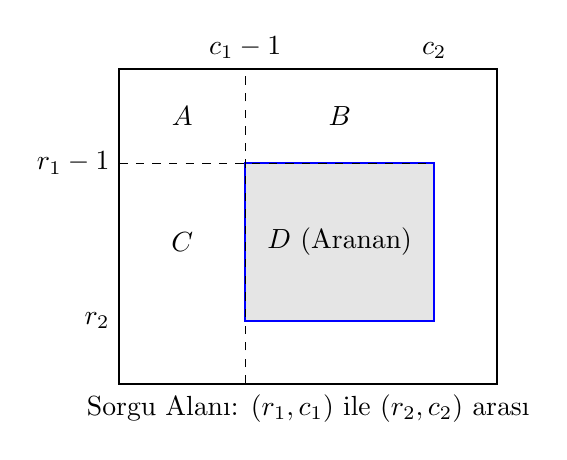
\begin{tikzpicture}[scale=0.8]
  % Büyük kutu
  \draw[thick] (0,0) rectangle (6,5);
  \node at (3, -0.4) {Sorgu Alanı: $(r_1, c_1)$ ile $(r_2, c_2)$ arası};
  
  % A, B, C, D alanları
  \fill[gray!20] (2,1) rectangle (5,3.5);
  \draw[thick, blue] (2,1) rectangle (5,3.5);
  \node at (3.5, 2.25) {$D$ (Aranan)};
  
  % Koordinat çizgileri
  \draw[dashed] (0, 3.5) -- (5, 3.5);
  \draw[dashed] (2, 0) -- (2, 5);
  
  \node[left] at (0, 3.5) {$r_1 - 1$};
  \node[left] at (0, 1) {$r_2$};
  \node[above] at (2, 5) {$c_1 - 1$};
  \node[above] at (5, 5) {$c_2$};
  
  \node at (1, 4.25) {$A$};
  \node at (3.5, 4.25) {$B$};
  \node at (1, 2.25) {$C$};
\end{tikzpicture}
\caption{2 Boyutlu Prefix Sums ve İçerme-Dışarma}
\end{figure}

Herhangi bir $[r_1 \dots r_2] \times [c_1 \dots c_2]$ sorgusunun toplamı:
\[
\text{Toplam} = P[r_2][c_2] - P[r_1 - 1][c_2] - P[r_2][c_1 - 1] + P[r_1 - 1][c_1 - 1].
\]

C dilinde 1-tabanlı indeksleme kullanarak sınır kontrollerini doğrudan sadeleştirebiliriz:

\begin{lstlisting}[language=CTemel]
#define MAXN 1005

long long P[MAXN][MAXN];

/* On hazirlik: O(N * M) zaman ve alan */
void on_hazirlik(int N, int M, int Matris[MAXN][MAXN]) {
    for (int i = 1; i <= N; i++) {
        for (int j = 1; j <= M; j++) {
            P[i][j] = Matris[i][j] 
                    + P[i - 1][j] 
                    + P[i][j - 1] 
                    - P[i - 1][j - 1];
        }
    }
}

/* Sorgu: O(1) zaman */
long long aralik_sorgusu(int r1, int c1, int r2, int c2) {
    return P[r2][c2] 
         - P[r1 - 1][c2] 
         - P[r2][c1 - 1] 
         + P[r1 - 1][c1 - 1];
}
\end{lstlisting}
Bu sayede her sorgu tam olarak 3 toplama/çıkarma işlemiyle $O(1)$ zamanda yanıtlanır.
\end{proof}

\subsection{İşaretçiler ve Bellek Takibi (Pointer Tracing)}

\begin{example}
Aşağıdaki C kod bloğu çalıştırıldığında ekrana basılacak çıktıyı adım adım bellek haritasını çizerek belirleyiniz.

\begin{lstlisting}[language=CTemel]
#include <stdio.h>

int main(void) {
    int a[] = {10, 20, 30, 40, 50};
    int *p = a;
    int *q = &a[3];
    
    printf("%ld\n", q - p);
    printf("%d\n", *p + *q);
    
    p += 2;
    printf("%d\n", *p);
    
    *p = *(p + 1) + 5;
    printf("%d\n", a[2]);
    
    return 0;
}
\end{lstlisting}
\end{example}

\begin{proof}[Çözüm]
C dilinde dizi isimleri ilk elemanın adresine dönüşür (decay). İşaretçi aritmetiğinde (Bölüm 31) adresler bayt cinsinden değil, işaret edilen veri türünün boyutu ($sizeof(T)$) cinsinden ölçeklenir. Bellek durumunu adım adım takip edelim:

\begin{enumerate}
    \item \textbf{İlk Durum:}
    \texttt{a} dizisi bellekte ardışık 5 tam sayı barındırır:
    \begin{itemize}
        \item \texttt{a[0] = 10} (Adres: $A$)
        \item \texttt{a[1] = 20} (Adres: $A + 1 \times 4$)
        \item \texttt{a[2] = 30} (Adres: $A + 2 \times 4$)
        \item \texttt{a[3] = 40} (Adres: $A + 3 \times 4$)
        \item \texttt{a[4] = 50} (Adres: $A + 4 \times 4$)
    \end{itemize}
    \texttt{p = a} $\implies p$, \texttt{a[0]} elemanını göstermektedir.
    \texttt{q = \&a[3]} $\implies q$, \texttt{a[3]} elemanını göstermektedir.

    \item \textbf{Birinci \texttt{printf}: \texttt{q - p}}
    İki işaretçi arasındaki fark, aralarındaki bayt farkı değil, \textbf{eleman sayısı} farkıdır:
    \[
    q - p = \&a[3] - \&a[0] = 3.
    \]
    Ekrana \textbf{3} yazılır.

    \item \textbf{İkinci \texttt{printf}: \texttt{*p + *q}}
    İşaretçilerin gösterdiği değerler toplanır:
    \texttt{*p = a[0] = 10}, \texttt{*q = a[3] = 40}.
    \[
    10 + 40 = 50.
    \]
    Ekrana \textbf{50} yazılır.

    \item \textbf{İşaretçi İlerlemesi: \texttt{p += 2}}
    $p$ işaretçisi 2 eleman ileri kaydırılır. Artık \texttt{p}, \texttt{a[2]} adresini gösterir.
    \texttt{printf("\%d\textbackslash\{\}n", *p)} $\implies$ \texttt{*p = a[2] = 30}.
    Ekrana \textbf{30} yazılır.

    \item \textbf{Değer Ataması: \texttt{*p = *(p + 1) + 5}}
    \texttt{p} şu anda \texttt{\&a[2]} adresindedir.
    \texttt{p + 1} ifadesi \texttt{\&a[3]} adresini gösterir.
    \texttt{*(p + 1)} değeri \texttt{a[3] = 40}'tır.
    Böylece \texttt{*p = 40 + 5 = 45} olur.
    \texttt{*p} doğrudan \texttt{a[2]} hücresini temsil ettiğinden, \texttt{a[2]} değeri $45$ olarak güncellenir.
    \texttt{printf("\%d\textbackslash\{\}n", a[2])} $\implies$ ekrana \textbf{45} yazılır.
\end{enumerate}

Kodun nihai çıktısı satır satır şöyledir:
\begin{verbatim}
3
50
30
45
\end{verbatim}
\end{proof}

\textbf{En sık yapılan hata:} \texttt{q - p} farkını hesaplarken bayt farkını (örneğin 32-bit \texttt{int} için $3 \times 4 = 12$) cevap olarak yazmaktır. C standardında işaretçi farkı daima aradaki eleman adedini (\texttt{ptrdiff\_t}) verir.

\subsection{Rekürsiyon ve Geriye İz Sürme (Backtracking)}

\begin{example}
$n$ basamaklı, yalnızca $\{1, 2, 3\}$ rakamlarından oluşan ve yan yana gelen hiçbir iki rakamın aynı olmadığı tüm sayıları sözlük sırasına (lexicographical order) göre ekrana basan rekürsif (rekürsif) C fonksiyonunu yazınız.
\end{example}

\begin{proof}[Çözüm]
Bu problem bir durum ağacını dolaşma yapısındadır (Bölüm 26). Her adımda elimizdeki sayıya eklenebilecek geçerli rakamları deneriz. Bir önceki adımda eklenen rakam ne ise, mevcut adımda o rakam dışındaki seçenekler sırayla denenir. Sözlük sırası istendiği için denemeleri küçük rakamdan büyüğe ($1 \to 2 \to 3$) doğru yapmalıyız. Taban durum (base case) basamak sayısı $n$'e ulaştığında sayıyı ekrana yazdırmaktır.

C dilinde bunu parametrik bir dizi (karakter katarı) ile geriye iz sürme (backtracking) yaparak kurabiliriz:

\begin{lstlisting}[language=CTemel]
#include <stdio.h>

/* dizi: mevcut sayiyi tutar
   basamak: su an doldurulacak indeks (0'dan n-1'e)
   n: hedeflenen basamak sayisi */
void olustur(char dizi[], int basamak, int n) {
    /* Taban durum: n basamak dolduruldu */
    if (basamak == n) {
        dizi[n] = '\0'; /* Katar sonlandirici */
        printf("%s\n", dizi);
        return;
    }
    
    /* 1, 2, 3 rakamlarini kucukten buyuge dene */
    for (char rakam = '1'; rakam <= '3'; rakam++) {
        /* Yan yana ayni rakam gelmeme kosulu */
        if (basamak == 0 || dizi[basamak - 1] != rakam) {
            dizi[basamak] = rakam;      /* Secimi yap */
            olustur(dizi, basamak + 1, n); /* Derine in */
            /* Geri donuste ekstra temizlige gerek yoktur,
               cunku sonraki dongu ayni indeksi ezecektir. */
        }
    }
}

void tum_sayilari_yazdir(int n) {
    char dizi[50]; /* n < 50 varsayilmistir */
    olustur(dizi, 0, n);
}
\end{lstlisting}

\textbf{Ağaç Boyutu ve Karmaşıklık:}
İlk basamak için 3 seçenek vardır. Sonraki her basamak için bir önceki basamaktan farklı 2 seçenek vardır. Toplam üretilen sayı adedi:
\[
3 \times 2^{n-1}
\]
olur. Her sayının basılması $O(n)$ sürdüğünden, toplam zaman karmaşıklığı $O(n \cdot 2^n)$ olur ve bu arama uzayı için asimptotik olarak optimaldir.
\end{proof}

\section{Bölüm Özeti ve İpuçları Kılavuzu}

Sınavda soru çözerken tıkandığınız anlarda aşağıdaki kontrol listesini zihninizden geçirebilirsiniz:

\begin{enumerate}
    \item \textbf{Küçük Değerler Yöntemi:} $n = 1, 2, 3, 4$ için elle yazıp tablo oluşturun. Çoğu kombinatorik ve sayı teorisi sorusunda genel kural küçük örneklerin örüntüsünden ortaya çıkar.
    \item \textbf{Simetri ve Tamlayıcı Sayma:} İstenen durumu doğrudan saymak karmaşıksa, tüm durumlardan istenmeyen durumları çıkarmayı (tümleyen küme, Bölüm 1 ve Bölüm 8) düşünün.
    \item \textbf{Uç Değer ve Uç Durumlar:} Algoritmada dizinin boş olması, $k=0$, tek eleman veya negatif sayılar gibi sınır durumları mutlaka test edin (Bölüm 19).
    \item \textbf{Karmaşıklık Bütçesi:} $N \le 10^5$ ise $O(N^2)$ çözümün zaman aşımı (TLE) alacağını göz önünde bulundurun; $O(N \log N)$ veya $O(N)$ arayışına girin (Bölüm 21). $N \le 20$ ise $O(2^N)$ geri iz sürme kabul edilebilir çözümdür.
\end{enumerate}
